\chapter{Results}
\label{chap:results}

\section*{}

This chapter reports several benchmarks analyzing the performance of several
algorithms, as well as benchmarks to analyze the influence of several
parameters of the \textit{MAX-MIN ant system}.

The first section, section~\ref{sec:aco}, presents the sensitivity analysis on
\textit{MAX-MIN ant system}'s parameters. It provides information that allows
one to balance the trade-off between route efficiency and running time.

Section~\ref{sec:results} presents the benchmark results that compare the
techniques described in the previous chapter when applied to the large
\textit{Asymmetric Capacitated Vehicle Routing Problem} datasets.

Unless specified otherwise, all benchmarks shown are obtained through averaging
ten runs for each algorithm/dataset. All running times were obtained by running
the algorithms on the same hardware and platform. The CPU was an
Intel\textsuperscript{\textregistered} Xeon\textsuperscript{\textregistered},
running at 2.33 GHz with 1 GB of RAM, running on the Ubuntu operating system, a
Linux distribution.






\section{Sensitivity of MAX-MIN ant system to algorithm parameters}
\label{sec:aco}

To understand how MMAS parameters influence the performance of the resulting
routes, there was the need to execute a series of benchmarks and comparisons.
These were done by varying the target parameter's value and by using the
validation datasets. This analysis will aid in configuring the parameters for
the application of this technique to larger datasets.

\newpage

\subsection{Parameter $\beta$ sensitivity}
\label{section:beta-sensitivity}

The first parameter whose influence was evaluated was $\beta$, a parameter that
measures the relative weight between an given arc distance and pheromone
intensity (Equation~\ref{eq:next-child}). The higher the $\beta$, the more ants
tend to choose shorter arcs and ignore pheromones. If $\beta$ is too high, the
pheromone intensity will be negligible, degenerating into the \textit{nearest
neighbor} heuristic.

To verify whether a correlation between the best $\beta$ and number of nodes
exists or not, this analysis was made using datasets of 35, 70 and 170 vertices,
available in the \textit{TSPLIB} library.

The number of ants to use in each dataset is equal to the number of nodes, as
suggested in \cite{Stutzle1997}. MMAS was ran for 200 iterations in each dataset
with $\beta$ values ranging from $0$ to $150$. The resulting average route cost
can be seen in Figure~\ref{fig:beta}.


\begin{figure}[h!]
  \centering
  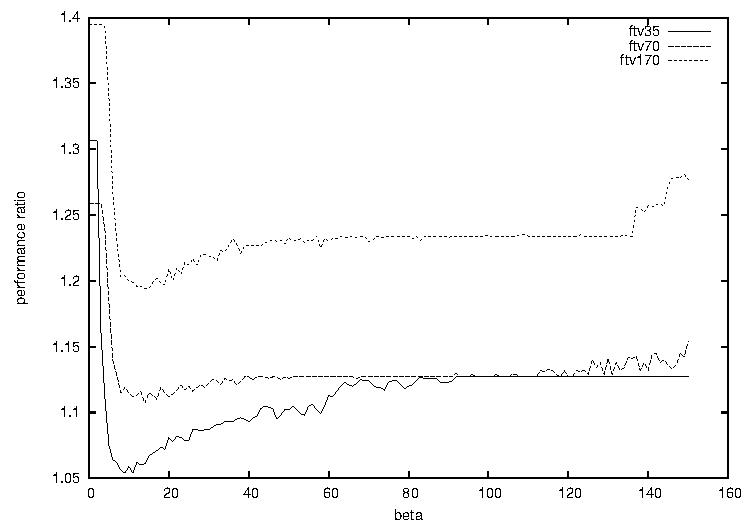
\includegraphics[width=0.80\textwidth]{beta}
  \caption{Variations in final route performance when varying beta in the
  MAX-MIN ant system for datasets ftv35, ftv70 and ftv170. Performance is given
  in the form of the ratio between the heuristic's route average cost and the
  dataset optimum (minimum) cost.}
  \label{fig:beta}
\end{figure}

We can observe that the best result for all datasets occurs for, approximately,
within the range $[5, 20]$. This is a good indicator that the optimum value for
$\beta$ is independent from the number of vertices in the graph.

The curve is steeper for $\beta$ values between $0$ and $5$. As such it was
decided to use $\beta=20$ in all subsequent executions, to prevent against
possible oscillations on the curve when dealing with larger graphs.






\newpage
\subsection{Trade-off between ants and iterations}
\label{section:mmas-tradeoff}

Having obtained a good reference for parameter $\beta$, the importance of the
number of ants and iterations was evaluated. Both of these parameters highly influence
the running time of the algorithm and the resulting route efficiency. As such,
it is important to determine what are the values for these two parameters that
yield more efficient routes within a limited time frame.

The first benchmark was done to verify if increasing the number of ants and
iterations produces more efficient routes. MMAS was applied to the larger of
the previous three datasets, \textit{ftv170}, with a varying number of ants for
$10000$ iterations and with $\beta=20$.  Figure~\ref{fig:mmas-ants-runs-small}
shows the results.

\begin{figure}[h!]
  \centering
  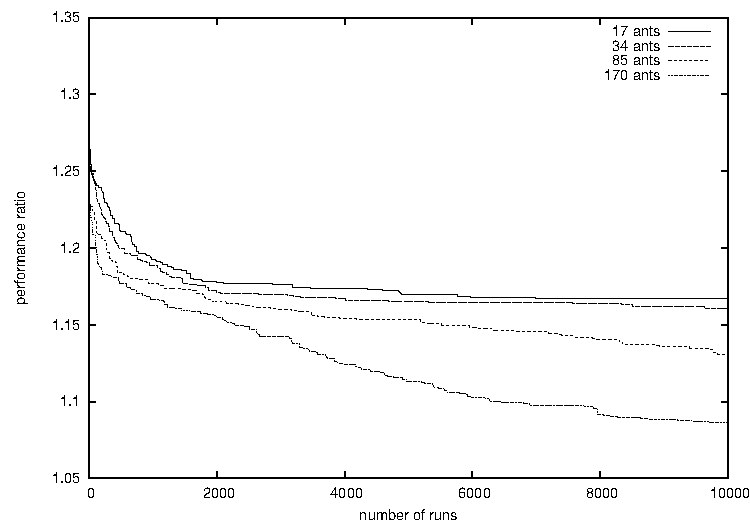
\includegraphics[width=0.80\textwidth]{ftv170-ant-comparison}
  \caption{Evolution of final route performance when varying the number of ants
  and number of iterations for the MAX-MIN ant system on dataset ftv170. Performance
  is given in the form of the ratio between the heuristic's route average cost
  and the dataset optimum (minimum) cost.}
  \label{fig:mmas-ants-runs-small}
\end{figure}

It becomes clear from the results that increasing both the number of ants and
the number of iterations --- as had been suggested by the original authors ---
improves the performance of the meta-heuristic.  It is important to verify if
the behavior presented in figure~\ref{fig:mmas-ants-runs-small} changes when the
number of nodes in the dataset increases. This was done by running additional
benchmarks with large datasets. Figure~\ref{fig:mmas-ants-runs-large} shows the
route cost evolution on a dataset with 1287 vertices, while
figure~\ref{fig:mmas-ants-runs-xl} shows this evolution on an even larger
dataset, with 6247 vertices.

\newpage
\begin{figure}[h!]
  \centering
  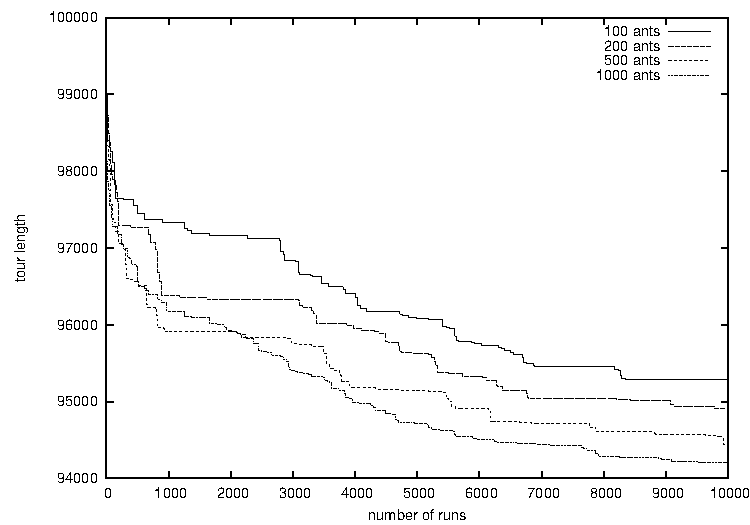
\includegraphics[width=0.8\textwidth]{hp1287-ant-comparison}
  \caption{Evolution of final tour length when varying the number of ants and
  number of iterations for the MAX-MIN ant system a dataset with 1287 vertices.}
  \label{fig:mmas-ants-runs-large}
\end{figure}

\begin{figure}[h!]
  \centering
  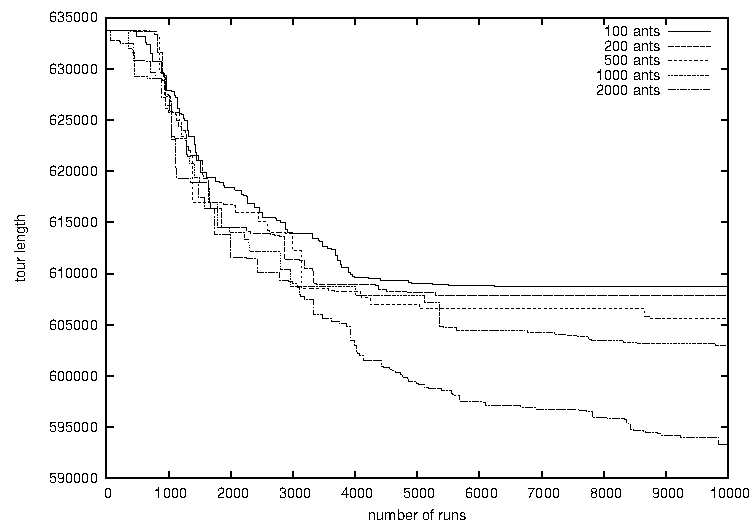
\includegraphics[width=0.8\textwidth]{hp6247-ant-comparison}
  \caption{Evolution of final tour length when varying the number of ants and
  number of iterations for the MAX-MIN ant system a dataset with 6247 vertices.}
  \label{fig:mmas-ants-runs-xl}
\end{figure}

The two figures~\ref{fig:mmas-ants-runs-large} and~\ref{fig:mmas-ants-runs-xl}
show that the behavior that occurred in figure~\ref{fig:mmas-ants-runs-small}
occurs, independently of the number of vertices in the graph. The difference in
the route efficiency, when varying the number of ants, is more prominent for
large number of iterations. The larger the dataset, the higher the number of
iterations has to be in order for this difference to be noticeable.

\newpage
It is worthy to notice that there is a trade-off between the computation time
and the efficiency of the obtained solution. Although all runs using the
dataset with 1287 vertices finished executing before a two hour limit, the
same was not true for the 6247 vertices dataset.
Table~\ref{tab:trade-off-hp6247} presents the average route efficiency when
varying the number of ants in dataset hp6247, after two hours of runtime.

\begin{table}[h!]
  \caption{Trade-off between running time and route efficiency, when varying the
  number of ants in dataset hp6247.}
  \begin{center}
    \begin{tabular}{rrr}
      \hline
      Number of ants & Average route cost & Average number of iterations \\
      \hline
       100 & 609056 & 6963 \\
       200 & 608310 & 4423 \\
       500 & 616919 & 1775 \\
      1000 & 629026 &  841 \\
      2000 & 632468 &  355 \\
      \hline
    \end{tabular}
  \end{center}
  \label{tab:trade-off-hp6247}
\end{table}



Although figure~\ref{fig:mmas-ants-runs-xl} shows that a higher number of ants
yields better results in the long run, table~\ref{tab:trade-off-hp6247} shows
that when given a limited time frame of two hours, it pays off to use a lower
number of ants.  Figure~\ref{fig:mmas-ants-runs-xl} also shows that the average
stagnation point of the $100$ ants curve occurs before the allowed number of
iterations within a two hour time-frame, so that the execution of the last runs
will bring no significant improvement. This explains why
table~\ref{tab:trade-off-hp6247} reports that runs with $200$ ants achieve, in
average, more efficient routes.

As a result of the sensibility analysis done in this section, it was concluded
that parameter $\beta$ should have a value around $20$. It was also shown that
when using small datasets --- or when the allowed running time is high --- it
pays off to use a higher number of ants. However, when applying MMAS to large
graphs within a limited time-frame, a lower number of ants achieves better
results.







\section{Algorithm performance on large ACVRP instances}
\label{sec:results}

To analyze the performance of the implemented algorithms when dealing with large
graphs, the seven techniques described in section~\ref{section:overview} were
applied to the large datasets presented in
section~\ref{section:realistic-datasets}.

Five of these seven techniques are \textit{route-first-cluster-second}
approaches, obtained through the application of one of the five ATSP methods ---
\textit{greedy} and \textit{repetitive nearest neighbor} heuristics,
\textit{hill climbing} (2-opt), a \textit{genetic algorithm} and \textit{MAX-MIN
ant system} --- followed by clustering using the \textit{split} algorithm. After
clustering, each of the resulting routes is subjected to the 2-opt algorithm
for further optimization.

The other two techniques are obtained through the application of the
Clarke-Wright's \textit{savings} heuristic, where each of the resulting routes
is optimized either by applying the 2-opt algorithm or MMAS.

The parameters for MMAS were chosen according to the sensibility analysis
presented in the previous section. All datasets were run with $\beta = 20$ and
$200$ ants for $3000$ iterations. Additionally, the length of the candidate
lists was set to $15$. The GA was executed with a population of $200$ for
$10000$ generations, so that its running time is close to the one of MMAS (see
the complexity analysis on section~\ref{section:complexity}). As explained in
section~\ref{section:genetic-algorithms}, this technique relies in mutations
only. 

All seven approaches can be divided into two main steps. The first step involves
finding a feasible CVRP solution, while the second step improves each of the
resulting routes by applying ATSP solutions. Furthermore, five of the seven
proposed approaches address the first step by further subdividing it into two
phases: finding an efficient ATSP solution for the whole graph (disregarding
capacity constraints) and clustering it into a feasible set of routes.

This section will present information regarding all of the three stages. As two
of the approaches do not rely on finding an initial ATSP solution, they will
only be analyzed on the two latter stages --- finding a CVRP solution and
optimizing each of its routes.

\subsection{ATSP solutions}
\label{section:large-atsp}

Table~\ref{tab:results-atsp} presents the average performance of the ATSP
approaches when applied to large datasets. The first four techniques
--- \textit{greedy}, \textit{repetitive nearest neighbor} and both 2-opt
algorithms --- are deterministic, so only one run of each was executed, as the
outcome would be always the same.

\begin{table}[h!]
  \caption{Performance of ATSP heuristic and meta-heuristic implementations
  using realistically large datasets. Minimum values for each dataset are
  highlighted.}
  \begin{center}
    \begin{tabular}{x{1.5cm} x{1.5cm} x{1.5cm} x{1.5cm} x{1.5cm} x{1.5cm} x{1.5cm} }
      \hline
  Vertices & Greedy &    RNN & RNN + 2-opt & Greedy + 2-opt &    GA &    MMAS \tabularnewline
      \hline
       518 &  64657 &  60967 &       58781 &          57911 &  58697 &  \textbf{53853} \tabularnewline
       841 &  83008 &  80964 &       78516 &          78226 &  77871 &  \textbf{76368} \tabularnewline
       904 &  93281 &  90415 &       87507 &          88594 &  87621 &  \textbf{80721} \tabularnewline
      1175 & 151028 & 157984 &      152446 &         139663 & 152172 & \textbf{138363} \tabularnewline
      1287 & 105806 &  99520 &       96348 &          97940 &  96468 &  \textbf{93179} \tabularnewline
      1849 & 193105 & 187885 &      183085 &         181541 & 182960 & \textbf{170317} \tabularnewline
      2038 & 221044 & 218138 &      211112 &         205540 & 211402 & \textbf{205131} \tabularnewline
      2206 & 210941 & 208363 &      202071 &         196331 & 202471 & \textbf{192239} \tabularnewline
      2561 & 489241 & 507214 &      495844 &         465692 & 495874 & \textbf{454568} \tabularnewline
      3481 & 514938 & 505256 &      492537 &         479361 & 492732 & \textbf{471214} \tabularnewline
      3859 & 513733 & 519371 &      505310 &         482014 & 505000 & \textbf{479331} \tabularnewline
      4109 & 531572 & 537033 &      528873 &         506615 & 529007 & \textbf{504745} \tabularnewline
      4628 & 586891 & 576868 &      563820 &         555597 & 564614 & \textbf{537557} \tabularnewline
      6247 & 639826 & 633747 &      623122 &         600162 & 623118 & \textbf{598762} \tabularnewline
      7628 & 699255 & 690216 &      676043 &         653948 & 676144 & \textbf{650564} \tabularnewline
      \hline
    \end{tabular}
  \end{center}
  \label{tab:results-atsp}
\end{table}

Table~\ref{tab:results-atsp} shows that MMAS achieves better results when
solving the ATSP for all of the large datasets. The proposed GA has a
performance similar to that of RNN 2-opt. In some datasets, 2-opt applied to the
greedy heuristic yields routes almost as efficient as MMAS. Additionally, it is
possible to calculate that the average improvement percentage of MMAS over all
15 datasets is of $2.6\%$, with a standard deviation of $2.5\%$.

To aid the comparison of the techniques, table~\ref{tab:mmas-improvement} shows
the values from table~\ref{tab:results-atsp} after a normalization process.
Normalization is done by dividing each value by the minimum value of its
dataset.

\begin{table}[h!]
  \caption{Normalized performance of ATSP techniques. Each value expressed as
  the percentage excess relative to the minimum value for its dataset.}
  \begin{center}
    \begin{tabular}{lx{1.5cm}x{1.5cm}x{1.5cm}x{1.5cm}x{1.5cm}x{1.5cm}}
      \hline
        & Greedy & RNN & Greedy + 2-opt & RNN + 2-opt & GA & MMAS \tabularnewline
      \hline
        & 20.1 \% & 13.2 \% & 7.5 \% &  9.2 \% &  9.0 \% & 0.0 \% \tabularnewline
        &  8.7 \% &  6.0 \% & 2.4 \% &  2.8 \% &  2.0 \% & 0.0 \% \tabularnewline
        & 15.6 \% & 12.0 \% & 9.8 \% &  8.4 \% &  8.5 \% & 0.0 \% \tabularnewline
        &  9.2 \% & 14.2 \% & 0.9 \% & 10.2 \% & 10.0 \% & 0.0 \% \tabularnewline
        & 13.6 \% &  6.8 \% & 5.1 \% &  3.4 \% &  3.5 \% & 0.0 \% \tabularnewline
        & 13.4 \% &  0.3 \% & 6.6 \% &  7.5 \% &  7.4 \% & 0.0 \% \tabularnewline
        &  7.8 \% &  6.3 \% & 0.2 \% &  2.9 \% &  3.1 \% & 0.0 \% \tabularnewline
        &  9.7 \% &  8.4 \% & 2.1 \% &  5.1 \% &  5.3 \% & 0.0 \% \tabularnewline
        &  7.6 \% & 11.6 \% & 2.4 \% &  9.1 \% &  9.1 \% & 0.0 \% \tabularnewline
        &  9.3 \% &  7.2 \% & 1.7 \% &  4.5 \% &  4.6 \% & 0.0 \% \tabularnewline
        &  7.2 \% &  8.4 \% & 0.6 \% &  5.4 \% &  5.4 \% & 0.0 \% \tabularnewline
        &  5.3 \% &  6.4 \% & 0.4 \% &  4.8 \% &  4.8 \% & 0.0 \% \tabularnewline
        &  9.2 \% &  7.3 \% & 3.4 \% &  4.9 \% &  5.0 \% & 0.0 \% \tabularnewline
        &  6.9 \% &  5.8 \% & 0.2 \% &  4.1 \% &  4.1 \% & 0.0 \% \tabularnewline
        &  7.5 \% &  6.1 \% & 0.5 \% &  3.9 \% &  3.9 \% & 0.0 \% \tabularnewline
      \hline
       $\mu$ & 10.1 \% &  8.7 \% &  2.9 \% &  5.7 \% &  5.7 \% & 0.0 \% \tabularnewline
$\sigma$ &  3.9 \% &  2.8 \% &  3.0 \% &  2.5 \% &  2.5 \% & 0.0 \% \tabularnewline
      \hline
    \end{tabular}
  \end{center}
  \label{tab:mmas-improvement}
\end{table}

Through the normalized values in table~\ref{tab:mmas-improvement}, it is easy to
see that the 2-opt algorithm with the greedy heuristic is the second best
approach to address the ATSP. These data also confirm that both the
\textit{genetic algorithm} and RNN 2-opt are similar.

\subsection{ACVRP solutions}
\label{section:large-atsp}

Although MMAS outperforms the other algorithms when solving the ATSP, it is not
guaranteed that it will outperform them when solving the ACVRP. To verify this,
the tours obtained in the previous sections were subjected to the clustering
algorithm described in section~\ref{section:clustering}. Additionally, the
\textit{savings} heuristic was also executed, so that
\textit{route-first-cluster-second} approaches could be compared to a
constructive heuristic for the CVRP.

The efficiency of each solution is given by the sum of each vehicle's route
length. The results for this run are in table~\ref{table:results-acvrp}. The
\textit{savings} heuristic is deterministic, so there was not the need to run it
more than once. The \textit{genetic algorithm} and \textit{max-min ant system}
had to be run multiple times, due to their stochastic nature.

\begin{table}[H]
  \caption{Performance of heuristic and meta-heuristic implementations using
  realistically large datasets. Minimum values for each dataset are
  highlighted.}
  \begin{center}
    \begin{tabular}{x{1.3cm} x{1.4cm} x{1.4cm} x{1.5cm} x{1.5cm} x{1.5cm}
    x{1.5cm} x{1.5cm} }
      \hline
Vertices &  Greedy &     RNN &  Greedy + 2-opt & RNN + 2-opt &      GA &    MMAS & Savings \tabularnewline
      \hline
     518 &   78072 &   77564 &           71521 &       75933 &   75448 &   \textbf{70640} &   93759 \tabularnewline
     841 &  114308 &  110422 &          109654 &      111192 &  107092 &  \textbf{104913} &  115576 \tabularnewline
     904 &  120087 &  120124 & \textbf{112396} &      117111 &  116067 &           113603 &  124092 \tabularnewline
    1175 &  223817 &  234530 &          224408 &      232428 &  232154 &  212875 &  \textbf{194312} \tabularnewline
    1287 &  133382 &  132784 & \textbf{125682} &      129607 &  129669 &           126473 &  152229 \tabularnewline
    1849 &  263830 &  273410 &          257318 &      263879 &  263935 &  249708 &  \textbf{238101} \tabularnewline
    2038 &  332029 &  333665 &          316529 &      317786 &  318345 &  304314 &  \textbf{281031} \tabularnewline
    2206 &  319361 &  325752 &          303652 &      313078 &  319353 &  304754 &  \textbf{291317} \tabularnewline
    2561 &  766226 &  777766 &          745094 &      767076 &  765974 &  \textbf{733627} &  831986 \tabularnewline
    3481 &  903800 &  905700 & \textbf{865213} &      894672 &  894868 &           876834 &  994299 \tabularnewline
    3859 &  910598 &  917740 &          880713 &      904655 &  903134 &  \textbf{879900} & 1040089 \tabularnewline
    4109 & 1062410 & 1071682 & \textbf{1038768} &    1062764 & 1062898 & 1044653 & 1193248 \tabularnewline
    4628 & 1099846 & 1104546 & \textbf{1067747} &    1091359 & 1095330 & 1070835 & 1245284 \tabularnewline
    6247 & 1381520 & 1379607 & \textbf{1339356} &    1369770 & 1369637 & 1353391 & 1639008 \tabularnewline
    7628 & 1579516 & 1595006 & \textbf{1537125} &    1577184 & 1577286 & 1556051 & 1912985 \tabularnewline
      \hline
    \end{tabular}
  \end{center}
  \label{table:results-acvrp}
\end{table}

Table~\ref{table:results-acvrp} shows that there is no direct relationship
between the ATSP solution efficiency and its respective ACVRP efficiency.
Nevertheless, MMAS yields more efficient routes in some of the datasets.  The
other two techniques that achieve the efficient routes for some datasets are the
2-opt algorithm, when used with the \textit{greedy} heuristic, and the
\textit{savings} construction heuristic.


Another important conclusion that the results on table~\ref{table:results-acvrp}
allow one to make is that although the \textit{greedy} heuristic has the lowest
performance on the ATSP, this gap is greatly reduced after applying the
clustering algorithm.

This is better described by quantifying the difference between algorithms when
transforming ATSP solutions to ACVRP solutions.
Table~\ref{table:results-atsp-vs-acvrp} shows, for each algorithm, the average
excess when compared to the best solution found for each dataset.


\begin{table}[H]
  \caption{Average route efficiency excess when comparing each algorithm to the
  best solution found for each dataset.}
  \begin{center}
    \begin{tabular}{rx{1.5cm}x{1.5cm}x{1.5cm}x{1.5cm}x{1.5cm}x{1.5cm}}
      \hline
       & Greedy &   RNN & Greedy + 2-opt & RNN + 2-opt & GA & MMAS \tabularnewline
      \hline
   ATSP & 10.1 \% & 8.7 \% & 2.9 \% & 5.7 \% & 5.7 \% & 0.0 \% \tabularnewline
  ACVRP &  7.3 \% & 8.1 \% & 3.2 \% & 6.1 \% & 5.9 \% & 2.2 \% \tabularnewline
      \hline
    \end{tabular}
  \end{center}
  \label{table:results-atsp-vs-acvrp}
\end{table}

Table~\ref{table:results-atsp-vs-acvrp} show that the \textit{greedy} has the
highest improvement, even surpassing the \textit{repetitive nearest neighbor}
heuristic. MMAS no longer dominates all the other algorithms (as shown in
table~\ref{table:results-acvrp}), but it is the algorithm with the lowest gap.




\subsection{Route improvement}
\label{section:route-improvement}

At this stage, each algorithm has already produced a feasible ACVRP solution,
composed of several routes. Each of the routes may be further optimized using
the previously mentioned ATSP techniques.

As shown in table~\ref{table:approach}, the six
\textit{route-first-cluster-second} approaches' solutions will be optimized
using the 2-opt improvement technique. On the other hand, the \textit{savings}
constructive heuristic will be optimized using two techniques: 2-opt and MMAS.
Table~\ref{tab:results-final} shows the final solution costs for all techniques.

\begin{table}[h!]
  \caption{Final ACVRP solutions' performance, after the application of the
  2-opt improvement technique. Minimum values for each dataset are
  highlighted.}
  \begin{center}
    \begin{tabular}{x{1.5cm} x{1.5cm} x{1.5cm} x{1.5cm} x{1.5cm} x{1.5cm}
    x{1.5cm} | x{1.5cm} }
      \hline
      \multicolumn{7}{c|}{2-opt improvement} & MMAS \tabularnewline
      \hline
 Greedy &    RNN &  Greedy + 2opt & RNN + 2-opt &    GA &    MMAS  & Savings &
 Savings \tabularnewline
\hline
  70534 &   74469 &   70588 &   74917 &   74422 &   \textbf{70161} &   91899 &   79032 \tabularnewline
 107288 &  103128 &  107304 &  106233 &  \textbf{102727} &  103291 &  112972 &  108669 \tabularnewline
 112511 &  111993 &  \textbf{109614} &  111479 &  113266 &  110986 &  120648 &  120223 \tabularnewline
 212389 &  225613 &  221932 &  230153 &  229544 &  208737 &  \textbf{189620} &  190846 \tabularnewline
 124957 &  128623 &  \textbf{124510} &  128624 &  128700 &  125161 &  149926 &  140379 \tabularnewline
 248255 &  264648 &  253844 &  259096 &  259068 &  247085 &  \textbf{233170} &  236821 \tabularnewline
 309866 &  323190 &  310721 &  312768 &  312855 &  300796 &  \textbf{276362} &  280927 \tabularnewline
 301713 &  312762 &  300303 &  306855 &  313087 &  301897 &  \textbf{284023} &  284310 \tabularnewline
 740730 &  764905 &  740815 &  763068 &  761945 &  \textbf{729603} &  823621 &  832580 \tabularnewline
 865570 &  887982 &  \textbf{859474} &  885902 &  885972 &  873044 &  975839 &  965098 \tabularnewline
 874926 &  896603 &  \textbf{871511} &  895631 &  893888 &  871832 & 1026658 &  987353 \tabularnewline
\textbf{1030661} & 1056671 & 1033678 & 1053607 & 1053741 & 1041138 & 1179891 & 1154823 \tabularnewline
1058717 & 1088214 & \textbf{1057246} & 1085945 & 1090055 & 1064012 & 1212899 & 1216222 \tabularnewline
1332414 & 1360244 & \textbf{1328719} & 1360440 & 1360441 & 1344851 & 1620740 & 1582320 \tabularnewline
\textbf{1518843} & 1565735 & 1520317 & 1562099 & 1562200 & 1544687 & 1894903 & 1840384 \tabularnewline
      \hline
    \end{tabular}
  \end{center}
  \label{tab:results-final}
\end{table}

The information on table~\ref{tab:results-final} shows that the minimum values
for each dataset are now scattered throughout the eight approaches. To help with
the analysis between the approaches, table~\ref{tab:results-final-normalized}
presents a normalization of these results.

\newpage
\begin{table}[H]
  \caption{Final ACVRP solutions' performance, after applying the final route
  optimization technique. Values are normalized by calculating the excess
  between a given algorithm's performance and the best value found for its
  dataset.}
  \begin{center}
    \begin{tabular}{rx{1.2cm} x{1.2cm} x{1.4cm} x{1.3cm} x{1.3cm} x{1.3cm}
    x{1.3cm} | x{1.5cm} }
      \hline
&     \multicolumn{7}{c|}{2-opt improvement} & MMAS \tabularnewline
      \hline
&  Greedy &    RNN &  Greedy + 2opt & RNN + 2-opt &    GA &    MMAS  & Savings &
 Savings \tabularnewline
\hline
&  0.5 \% &  6.1 \% &  0.6 \% &  6.8 \% &  6.1 \% &  0.0 \% & 31.0 \% & 12.6 \% \tabularnewline
&  4.4 \% &  0.4 \% &  4.5 \% &  3.4 \% &  0.0 \% &  0.5 \% & 10.0 \% &  5.8 \% \tabularnewline
&  2.6 \% &  2.2 \% &  0.0 \% &  1.7 \% &  3.3 \% &  1.3 \% & 10.1 \% &  9.7 \% \tabularnewline
& 12.0 \% & 19.0 \% & 17.0 \% & 21.4 \% & 21.1 \% & 10.1 \% &  0.0 \% &  0.6 \% \tabularnewline
&  0.4 \% &  3.3 \% &  0.0 \% &  3.3 \% &  3.4 \% &  0.5 \% & 20.4 \% & 12.7 \% \tabularnewline
&  6.5 \% & 13.5 \% &  8.9 \% & 11.1 \% & 11.1 \% &  6.0 \% &  0.0 \% &  1.6 \% \tabularnewline
& 12.1 \% & 16.9 \% & 12.4 \% & 13.2 \% & 13.2 \% &  8.8 \% &  0.0 \% &  1.7 \% \tabularnewline
&  6.2 \% & 10.1 \% &  5.7 \% &  8.0 \% & 10.2 \% &  6.3 \% &  0.0 \% &  0.1 \% \tabularnewline
&  1.5 \% &  4.8 \% &  1.5 \% &  4.6 \% &  4.4 \% &  0.0 \% & 12.9 \% & 14.1 \% \tabularnewline
&  0.7 \% &  3.3 \% &  0.0 \% &  3.1 \% &  3.1 \% &  1.6 \% & 13.5 \% & 12.3 \% \tabularnewline
&  0.4 \% &  2.9 \% &  0.0 \% &  2.8 \% &  2.6 \% &  0.0 \% & 17.8 \% & 13.3 \% \tabularnewline
&  0.0 \% &  2.5 \% &  0.3 \% &  2.2 \% &  2.2 \% &  1.0 \% & 14.5 \% & 12.0 \% \tabularnewline
&  0.1 \% &  2.9 \% &  0.0 \% &  2.7 \% &  3.1 \% &  0.6 \% & 14.7 \% & 15.0 \% \tabularnewline
&  0.3 \% &  2.4 \% &  0.0 \% &  2.4 \% &  2.4 \% &  1.2 \% & 22.0 \% & 19.1 \% \tabularnewline
&  0.0 \% &  3.1 \% &  0.1 \% &  2.8 \% &  2.9 \% &  1.7 \% & 24.8 \% & 21.2 \% \tabularnewline
 \hline
$\mu$ &  3.2 \% &  6.2 \% &  3.4 \% &  6.0 \% &  5.9 \% &  2.6 \% & 12.8 \% & 10.1 \% \tabularnewline
$\sigma$ &  4.2 \% &  5.8 \% &  5.4 \% &  5.5 \% &  5.6 \% &  3.4 \% &  9.7 \% &  6.7 \% \tabularnewline
      \hline
    \end{tabular}
  \end{center}
  \label{tab:results-final-normalized}
\end{table}

From table~\ref{tab:results-final-normalized}, one can see that although it does
not achieve the minimum for many datasets, MMAS has the highest performance
ratio ($2.6\%$). It also has the smallest standard deviation ($3.4\%$). This
makes it the most stable algorithm --- of those studied --- to solve the ACVRP
on the sample datasets.

Although the \textit{savings} heuristic followed by a 2-opt improvement produces
efficient routes for some of the datasets, it has a poor average performance
ratio. The \textit{savings} heuristic followed by MMAS has a better performance,
with a lower average excess gap and reduced standard deviation.

The second best algorithm, when taking these metrics into consideration, is the
\textit{greedy heuristic}. This shows that the CVRP performance of an algorithm
does not strictly depend on its performance on the ATSP.
Table~\ref{table:results-summary} summarizes the average performance for each
algorithm, in each of the three steps.

\begin{table}[H]
  \caption{Summary of the several techniques' performance, over the three
  optimization stages.}
  \begin{center}
    \begin{tabular}{rx{1.2cm}x{1.1cm}x{1.2cm}x{1.2cm}x{1.1cm}x{1.2cm}x{1.3cm}x{1.5cm}}
      \hline
       & Greedy &   RNN & Greedy + 2-opt & RNN + 2-opt & GA & MMAS & Savings & Savings + MMAS \tabularnewline
      \hline
   ATSP & 10.1 \% & 8.7 \% & 2.9 \% & 5.7 \% & 5.7 \% & 0.0 \% & -       & - \tabularnewline
  ACVRP &  7.3 \% & 8.1 \% & 3.2 \% & 6.1 \% & 5.9 \% & 2.2 \% & 13.3 \% & 13.3 \% \tabularnewline
  Final &  3.2 \% & 6.2 \% & 3.4 \% & 6.0 \% & 5.9 \% & 2.6 \% & 12.8 \% & 10.1 \% \tabularnewline
      \hline
    \end{tabular}
  \end{center}
  \label{table:results-summary}
\end{table}





\section{Chapter summary}
\label{section:results-summary}

This chapter presented the sensitivity analysis for the \textit{MAX-MIN ant
system}, regarding three parameters: $\beta$, number of ants and number of
iterations. This chapter also exposed results regarding the application of the
eight ACVRP techniques to large datasets.

Next chapter finalizes this document by presenting an overview of all the
conclusions made throughout this project --- both related to the algorithm
comparison and to the waste collection optimization framework.



